\documentclass[10pt]{article}
% Layout close to NeurIPS (single column, 5.5 in text width, 9 in text height, Times).
% For submission, replace this preamble with the official neurips_2026.sty template.
\usepackage[letterpaper,top=1in,bottom=1in,left=1.5in,right=1.5in]{geometry}
\usepackage{times}
\usepackage{amsmath,amssymb}
\usepackage{booktabs}
\usepackage{graphicx}
\usepackage[font=small,labelfont=bf,skip=3pt]{caption}
\usepackage{enumitem}
\usepackage[hidelinks]{hyperref}
\setlist{nosep,leftmargin=*}
\setlength{\parskip}{3pt}
\graphicspath{{../figures/}}
\newcommand{\R}{\mathbb{R}}
\newcommand{\abs}[1]{\lvert #1 \rvert}

\title{Estimating Sparse Precision Matrices:\\Graphical Lasso, Neighbourhood Selection, and a Reweighted Extension}
\author{Rishita Parashar (26M2009)\qquad Tanishq Sahu (26M2018)\\[2pt]
SC 663: Optimization and Inference in Sparse Network Models}
\date{}

\begin{document}
\maketitle

\begin{abstract}
We estimate the dependency network of Gaussian data from its precision matrix $Q$. We compare two estimators, the graphical lasso and neighbourhood selection with the AND rule, on simulated networks with known truth (Part A). On real protein data from Sachs et al.\ (Part B), we choose the penalty by simulation, check stability over random halves, and test trust by re-simulation. For the extension (Part C2) we derive a reweighted graphical lasso for the log-sum penalty by majorization--minimization. At matched sparsity it finds more true edges and reduces the shrinkage bias on true edges from $-0.33$ to $-0.05$.
\end{abstract}

\section{Problem}
Let $x_1,\dots,x_N\in\R^p$ be i.i.d.\ from $\mathcal N(0,Q^{-1})$. Variables $i$ and $j$ are conditionally independent given the rest exactly when $q_{ij}=0$, so the network is $E=\{(i,j): q_{ij}\neq 0\}$. When $p$ is large relative to $N$, $Q$ must be estimated under sparsity. We study two estimators:
\begin{itemize}
\item \textbf{Graphical lasso} \cite{friedman2008}: $\min_{Q\succ 0}\ -\log\det Q+\operatorname{tr}(SQ)+\lambda\sum_{i\neq j}\abs{q_{ij}}$, where $S$ is the sample covariance. Solved with scikit-learn.
\item \textbf{Neighbourhood selection} \cite{meinshausen2006}: for each node $j$, a lasso regression $\min_\beta \frac{1}{2N}\|x_j-X_{-j}\beta\|^2+\lambda\|\beta\|_1$ gives neighbours $k$ with $\beta_{jk}\neq 0$. The AND rule keeps $(j,k)$ only if both $\beta_{jk}\neq 0$ and $\beta_{kj}\neq 0$. Our own coordinate-descent lasso solver is checked against scikit-learn (maximum difference $3\times10^{-12}$).
\end{itemize}
Performance measures: $\mathrm{TPR}=\mathrm{TP}/\abs{E}$, $\mathrm{FPR}=\mathrm{FP}/(\binom{p}{2}-\abs{E})$, $F_1=2\mathrm{TP}/(2\mathrm{TP}+\mathrm{FP}+\mathrm{FN})$.

\section{Part A: simulation with known truth}
\textbf{Setup.} We use $p=60$ and two networks: Erd\H{o}s--R\'enyi with edge probability $0.05$ (67 edges) and a chain $i\!-\!(i{+}1)$ (59 edges). For each network we build $Q$ by two generators from the October 30 lecture: diagonal dominance (DD) and partial orthogonalization (PO). Each $Q$ is shifted so that $\lambda_{\min}(Q)=0.1$, which makes the two generators comparable. Data are drawn for $N\in\{40,100,200\}$ ($N=40<p$). Both estimators are run on $\lambda=r\lambda_{\max}$ with 25 values of $r$ from $1$ to $0.01$, where $\lambda_{\max}=\max_{j\neq k}\abs{S_{jk}}$. Each setting is repeated 35 times with fresh data, and TPR and FPR are averaged at each $\lambda$.

\textbf{Edge strength.} Table~\ref{tab:q} reports $\abs{\tilde q_{ij}}=\abs{q_{ij}}/\sqrt{q_{ii}q_{jj}}$ on the true edges. DD gives strong edges, and PO gives edges about half as strong.

\begin{table}[h]
\centering\small
\caption{Edge strengths $|\tilde q_{ij}|$ of the four precision matrices.}\label{tab:q}
\begin{tabular}{llrrrr}
\toprule
Network & Q & Edges & Mean & Median & Range\\
\midrule
ER & DD & 67 & 0.32 & 0.33 & 0.00--0.86\\
ER & PO & 67 & 0.20 & 0.15 & 0.00--0.89\\
Chain & DD & 59 & 0.42 & 0.44 & 0.02--0.78\\
Chain & PO & 59 & 0.17 & 0.13 & 0.00--0.85\\
\bottomrule
\end{tabular}
\end{table}

\begin{figure}[h]
\centering
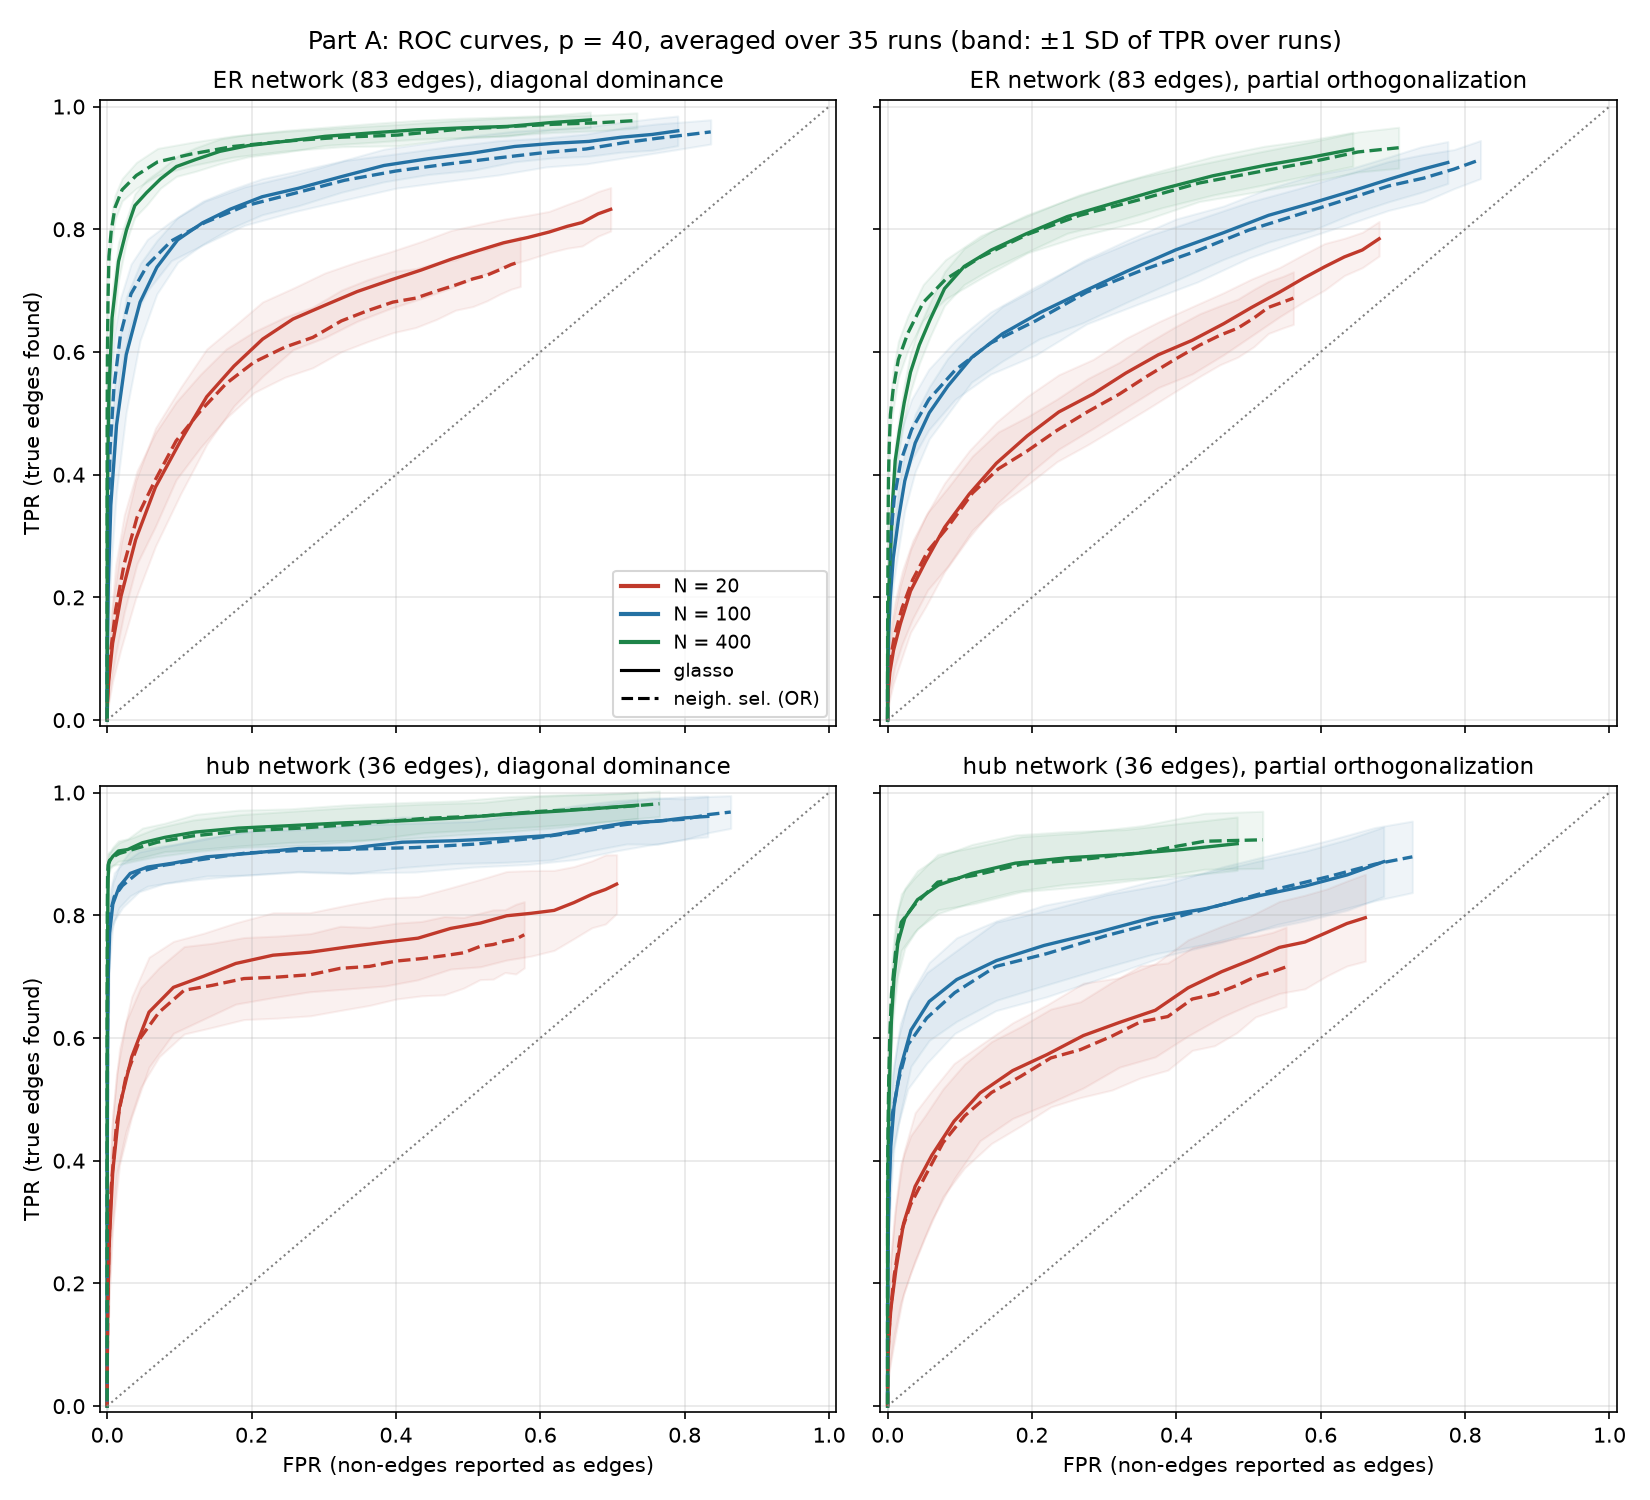
\includegraphics[width=0.8\linewidth]{partA_roc.png}
\caption{Averaged ROC curves (35 runs). Rows: network; columns: Q method; colour: $N$; solid: glasso; dashed: neighbourhood selection (AND); band: $\pm1$ SD of TPR. Closer to the top-left is better.}\label{fig:roc}
\end{figure}

\textbf{Results.} Table~\ref{tab:roc} gives the TPR at FPR $=0.05$ read off the averaged curves, as ``glasso / AND''.

\begin{table}[h]
\centering\small
\caption{TPR at FPR $=0.05$ (glasso / neighbourhood selection with AND), 35 runs.}\label{tab:roc}
\begin{tabular}{llccc}
\toprule
Network & Q & $N=40$ & $N=100$ & $N=200$\\
\midrule
ER & DD & 0.66 / 0.67 & 0.80 / 0.81 & 0.86 / 0.86\\
ER & PO & 0.32 / 0.34 & 0.44 / 0.47 & 0.55 / 0.57\\
Chain & DD & 0.77 / 0.79 & 0.88 / 0.90 & 0.92 / 0.94\\
Chain & PO & 0.20 / 0.23 & 0.35 / 0.39 & 0.46 / 0.52\\
\bottomrule
\end{tabular}
\end{table}

\textbf{Discussion: which estimator, under which conditions.}
\begin{itemize}
\item \emph{Edge strength is the dominant factor.} Going from DD to PO costs both estimators $0.3$--$0.6$ TPR at FPR $=0.05$. Weak edges are hard for any method.
\item \emph{Sample size.} Both estimators improve steadily with $N$. At $N=40$ (below $p$), the graphical lasso has the higher curve for strong edges once FPR exceeds about $0.05$; the AND curve stops early at FPR $\approx 0.35$. A plausible reason is that each node's lasso can select at most $N$ neighbours, which caps the AND graph's density. We have not tested this directly.
\item \emph{Weak edges and larger $N$.} For PO, the AND rule is ahead at every $N$, and the gap grows with $N$ (0.02 at $N=40$, up to 0.06 on the chain at $N=200$). Differences are often within one SD, so this is a tendency, not a firm ranking.
\item \emph{Network type.} With DD edges the chain is easier for both estimators (+0.06 to +0.12 TPR than ER). With PO edges it is harder (-0.05 to -0.12). The sign follows the difference in edge strength (chain DD edges are stronger, PO edges weaker), so network type acts mainly through edge strength.
\end{itemize}
In short, the estimators are close. The AND rule is at least as good as glasso for weak edges and $N\ge 100$, and the glasso is better at $N=40$.

\section{Part B: real data (Sachs protein signalling)}
\textbf{Data and preprocessing.} We use 7,466 cells and 11 phosphoproteins from Sachs et al.\ \cite{sachs2005}. Measurements are right-skewed, so we take logs and standardise each variable. The 20-edge literature skeleton is used only for evaluation.

\textbf{Choosing $\lambda$ by simulation.} We draw 20 data sets with the same $p=11$ and $N=7{,}466$ from a precision matrix (DD) whose network is the 20-edge skeleton. For each relative value $r$ we compute the average F$_1$ and keep the best $r$. The glasso chooses $r=0.056$ (mean F$_1$ 0.89) and the AND estimator chooses $r=0.026$ (mean F$_1$ 0.95).

\textbf{Stability and stable edges.} We take 50 random halves (3,733 samples each) and rerun each estimator with the chosen $r$. The selection frequency of a pair is the share of halves where it is an edge. Edges with frequency at least $80\%$ are stable; Figure~\ref{fig:sel} shows the frequencies. The glasso gives 34 stable edges and AND gives 32.

\begin{figure}[h]
\centering
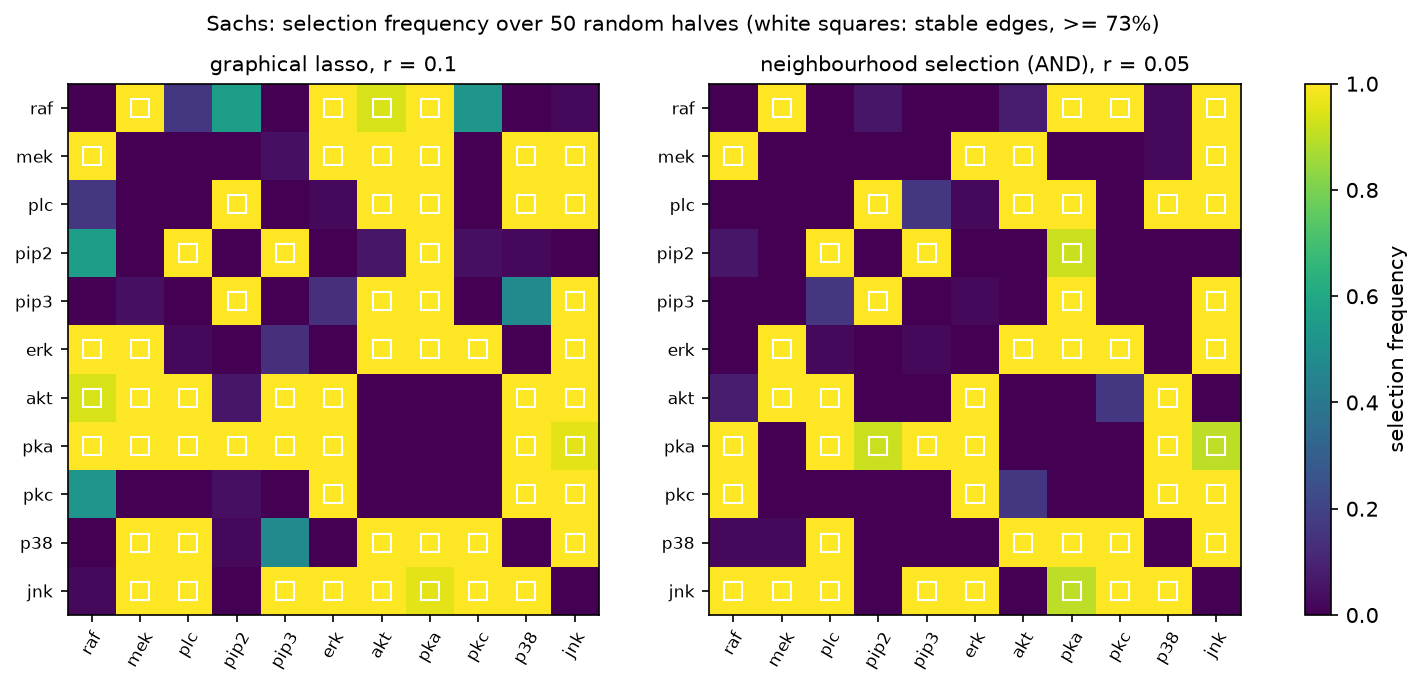
\includegraphics[width=0.95\linewidth]{partB_selection.png}
\caption{Selection frequency over 50 random halves for each estimator. Red circles mark the 20 skeleton edges.}\label{fig:sel}
\end{figure}

\textbf{Comments on edges.} Pairs such as \texttt{raf--mek} and \texttt{mek--erk} are selected in every half and are in the skeleton; they are consecutive steps of the MAPK cascade, which is a direct biological link. \texttt{plc--pip2} is also stable and in the skeleton, consistent with PLC hydrolysing PIP$_2$. \texttt{raf--jnk} is selected in every half but is not in the skeleton. Both \texttt{raf} and \texttt{jnk} are regulated by \texttt{pka} and \texttt{pkc}, so this may be an indirect association rather than a direct link.

\textbf{Trust.} We take the stable network as the truth. Its edge strengths come from the glasso precision on all the data, restricted to the stable edges and rescaled to unit diagonal (positive definite in both cases). We simulate 20 data sets with the same $p$ and $N$ and estimate them with the same relative $\lambda$ (Table~\ref{tab:trust}).

\begin{table}[h]
\centering\small
\caption{Summary of the Sachs analysis. Trust columns are mean $\pm$ SD over 20 simulated data sets.}\label{tab:trust}
\begin{tabular}{lcccc}
\toprule
Estimator & $r$ & Stable edges & TPR & FPR\\
\midrule
Graphical lasso & 0.056 & 34 & $0.83\pm0.03$ & $0.190\pm0.044$\\
Neighbourhood (AND) & 0.026 & 32 & $0.81\pm0.03$ & $0.026\pm0.026$\\
\bottomrule
\end{tabular}
\end{table}

On the real data, the glasso selects 36 edges (F$_1$ 0.50 against the skeleton) and AND selects 34 (F$_1$ 0.56). In the trust simulation, AND produces far fewer false edges (FPR 0.03 against 0.19) at the same TPR. This agrees with Part A: AND is more conservative. We therefore report the AND network as the main result, with the caveat that the Sachs data pool observational and interventional cells, and the skeleton is only a literature reference.

\section{Part C2: reweighted graphical lasso (log-sum penalty)}
\textbf{Problem.} The $\ell_1$ penalty shrinks large and small entries equally, so strong true edges are underestimated. We replace it with the log-sum penalty:
\[
F(Q)=\ell(Q;S)+\lambda\sum_{i\neq j}\log\bigl(\abs{q_{ij}}+\varepsilon\bigr),\qquad \ell(Q;S)=-\log\det Q+\operatorname{tr}(SQ),\quad \varepsilon>0.
\]

\textbf{Derivation (majorization--minimization).} The function $g(t)=\log(t+\varepsilon)$ is concave on $t\ge0$, so it lies below its tangent at any point $t_0\ge 0$:
\[
\log(t+\varepsilon)\le \log(t_0+\varepsilon)+\frac{t-t_0}{t_0+\varepsilon}.
\]
Put $t=\abs{q_{ij}}$ and $t_0=\abs{q^{(k)}_{ij}}$. Summing over $i\neq j$ gives a surrogate $G_k(Q)\ge F(Q)$ that is equal to $F$ at $Q^{(k)}$:
\[
G_k(Q)=\ell(Q;S)+\lambda\sum_{i\neq j}w^{(k)}_{ij}\abs{q_{ij}}+\text{const},\qquad w^{(k)}_{ij}=\frac{1}{\abs{q^{(k)}_{ij}}+\varepsilon}.
\]
Let $Q^{(k+1)}=\arg\min_{Q\succ0}G_k(Q)$, the weighted graphical lasso. Then
\[
F(Q^{(k+1)})\le G_k(Q^{(k+1)})\le G_k(Q^{(k)})=F(Q^{(k)}),
\]
so $F$ never increases. Large entries receive small weights (little shrinkage), and small entries receive large weights (pushed to zero).

\textbf{Algorithm.} We start from the ordinary glasso, then iterate the weighted glasso for up to 5 steps. We solve each weighted glasso by block coordinate descent \cite{friedman2008}, where each column update is a lasso with per-coefficient weights, solved by rescaling into a standard lasso. With unit weights our solver agrees with scikit-learn to $2\times10^{-5}$ with the same support, and $F$ decreased monotonically in the tests.

\textbf{Experiment.} We use the chain network with DD precision matrix, $N=100$, and 35 runs (the same data as Part A). The reweighted fit uses $\lambda$ chosen by BIC, and the glasso uses the $\lambda$ that gives the closest number of edges, so both have about the same sparsity. Bias is $\frac{1}{\abs E}\sum_{(i,j)\in E}(\abs{\hat q_{ij}}-\abs{q_{ij}})$.

\begin{table}[h]
\centering\small
\caption{Glasso and reweighted glasso at matched sparsity (chain, DD, $N=100$, 35 runs).}\label{tab:c2}
\begin{tabular}{lcccc}
\toprule
Method & Edges & TPR & F$_1$ & Bias\\
\midrule
Glasso & $56\pm8$ & $0.74\pm0.05$ & $0.76\pm0.04$ & $-0.331\pm0.015$\\
Reweighted & $57\pm5$ & $0.87\pm0.03$ & $0.88\pm0.04$ & $-0.051\pm0.011$\\
\bottomrule
\end{tabular}
\end{table}

\begin{figure}[h]
\centering
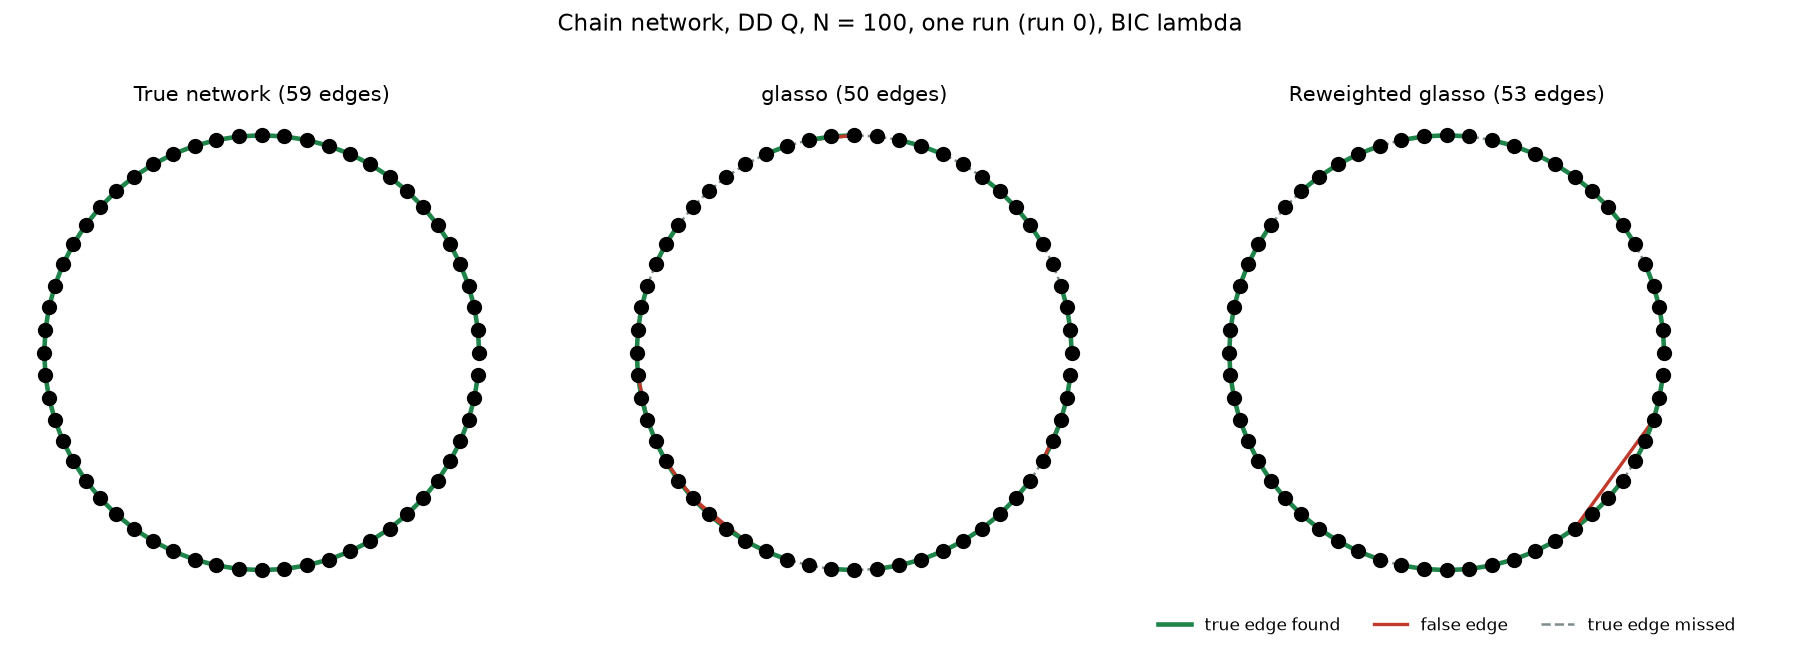
\includegraphics[width=0.95\linewidth]{partC2_network.png}
\caption{One run (BIC $\lambda$, matched sparsity). Green: true edge found; red: false edge; dashed grey: true edge missed.}\label{fig:net}
\end{figure}

\begin{figure}[h]
\centering
\begin{minipage}[t]{0.52\linewidth}\centering
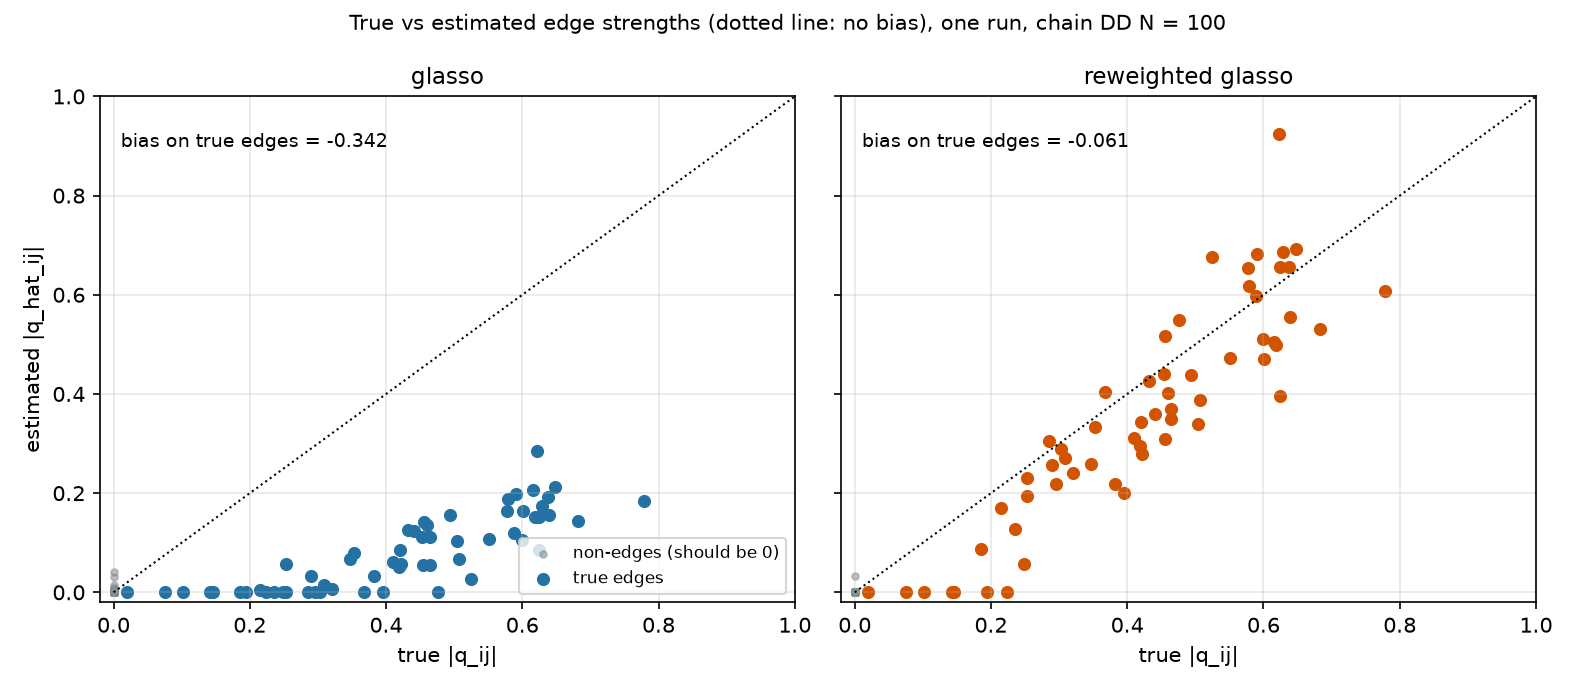
\includegraphics[width=\linewidth]{partC2_strength.png}\\[-2pt]
{\small (a) true vs estimated $|q|$}
\end{minipage}\hfill
\begin{minipage}[t]{0.44\linewidth}\centering
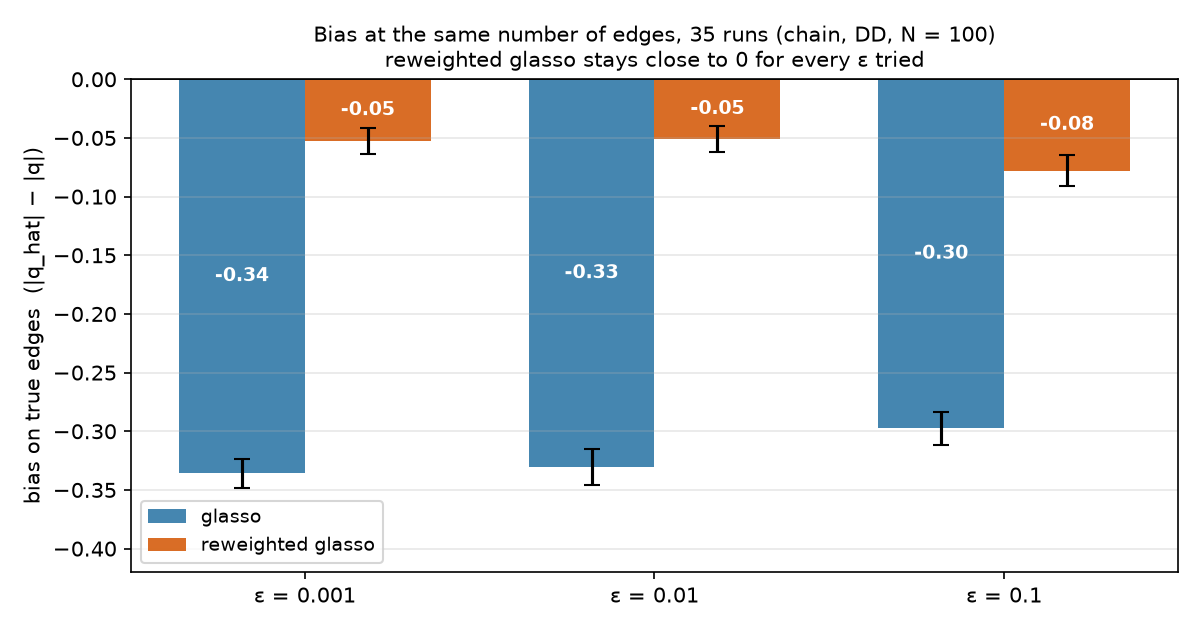
\includegraphics[width=\linewidth]{partC2_bias_eps.png}\\[-2pt]
{\small (b) bias for $\varepsilon\in\{0.001,0.01,0.1\}$}
\end{minipage}
\caption{(a) Estimated against true edge strengths for one run; points on the dotted line have no bias. (b) Bias across $\varepsilon$ (35 runs). Reweighted bias stays near $-0.05$ for $\varepsilon\le 0.01$ and is $-0.08$ at $\varepsilon=0.1$, where the result is weaker (F$_1$ 0.78 against 0.88).}\label{fig:bias}
\end{figure}

\textbf{Results.} At matched sparsity the reweighted estimator finds more true edges (TPR 0.87 against 0.74) with a similar number of edges, and its bias is about six times smaller. The conclusion holds for $\varepsilon=0.001$ and $0.01$ (F$_1$ 0.90 and 0.88 against 0.76). With $\varepsilon=0.1$ the penalty is closer to the $\ell_1$ penalty and the gain is smaller.

\section{Discussion and limitations}
Our results cover two network types at one dimension ($p=60$), two generators, and sample sizes $40$--$200$. We did not test hub networks, $N=400$, or edges weaker than PO. The Part C2 comparison uses one setting. MM converges only to a local solution, so we start from the glasso fit. Part B uses the Sachs skeleton both to choose $\lambda$ and to judge the result, which is a simplification. Part C1 (differential networks) was not attempted.

\section*{Contributions}
Rishita Parashar: Part A (simulation, both estimators, solvers, figures) and Part C (reweighted glasso derivation and experiment). Tanishq Sahu: Part B (Sachs analysis, stability and trust).

\section*{Use of Gen-AI tools}
We used Claude (Anthropic) to draft and debug Python code, to check the algebra of the MM derivation, and to help write this LaTeX source. All experiments were run by us, and every number in this report was taken from the saved output files in the repository.

\begin{thebibliography}{9}
\bibitem{friedman2008} J.~Friedman, T.~Hastie, R.~Tibshirani. Sparse inverse covariance estimation with the graphical lasso. \emph{Biostatistics}, 2008.
\bibitem{meinshausen2006} N.~Meinshausen, P.~B\"uhlmann. High-dimensional graphs and variable selection with the lasso. \emph{Ann.\ Statist.}, 2006.
\bibitem{cordoba2020} I.~C\'ordoba, G.~Varando, C.~Bielza, P.~Larra\~naga. On generating random Gaussian graphical models. \emph{Int.\ J.\ Approx.\ Reasoning}, 2020.
\bibitem{sachs2005} K.~Sachs et al. Causal protein-signaling networks derived from multiparameter single-cell data. \emph{Science}, 2005.
\bibitem{candes2008} E.~J.~Cand\`es, M.~B.~Wakin, S.~Boyd. Enhancing sparsity by reweighted $\ell_1$ minimization. \emph{J.\ Fourier Anal.\ Appl.}, 2008.
\end{thebibliography}
\end{document}
